\documentclass[dvipdfmx]{jarticle}
\pagestyle{empty}
\usepackage{tikz}
\usetikzlibrary{calc,shapes,arrows.meta}
\begin{document}
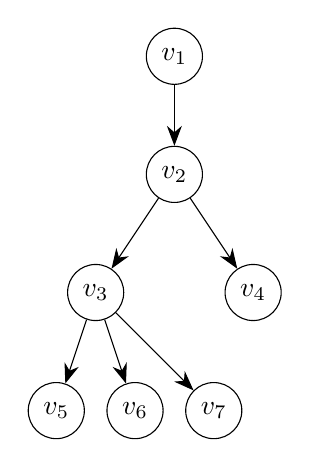
\begin{tikzpicture}
\node[draw,circle] (N1) at (0,0) {$v_1$};
\node[draw,circle] (N2) at (0,-1.5) {$v_2$};
\node[draw,circle] (N3) at (-1,-3) {$v_3$};
\node[draw,circle] (N4) at (1,-3) {$v_4$};
\node[draw,circle] (N5) at (-1.5,-4.5) {$v_5$};
\node[draw,circle] (N6) at (-0.5,-4.5) {$v_6$};
\node[draw,circle] (N7) at (0.5,-4.5) {$v_7$};
\path[-{Stealth[scale=1.5]}] (N1) edge (N2);
\path[-{Stealth[scale=1.5]}] (N2) edge (N3) (N2) edge (N4);
\path[-{Stealth[scale=1.5]}] (N3) edge (N5) (N3) edge (N6) (N3) edge (N7);
\end{tikzpicture} 
\end{document}